\begin{figure*}
\centering
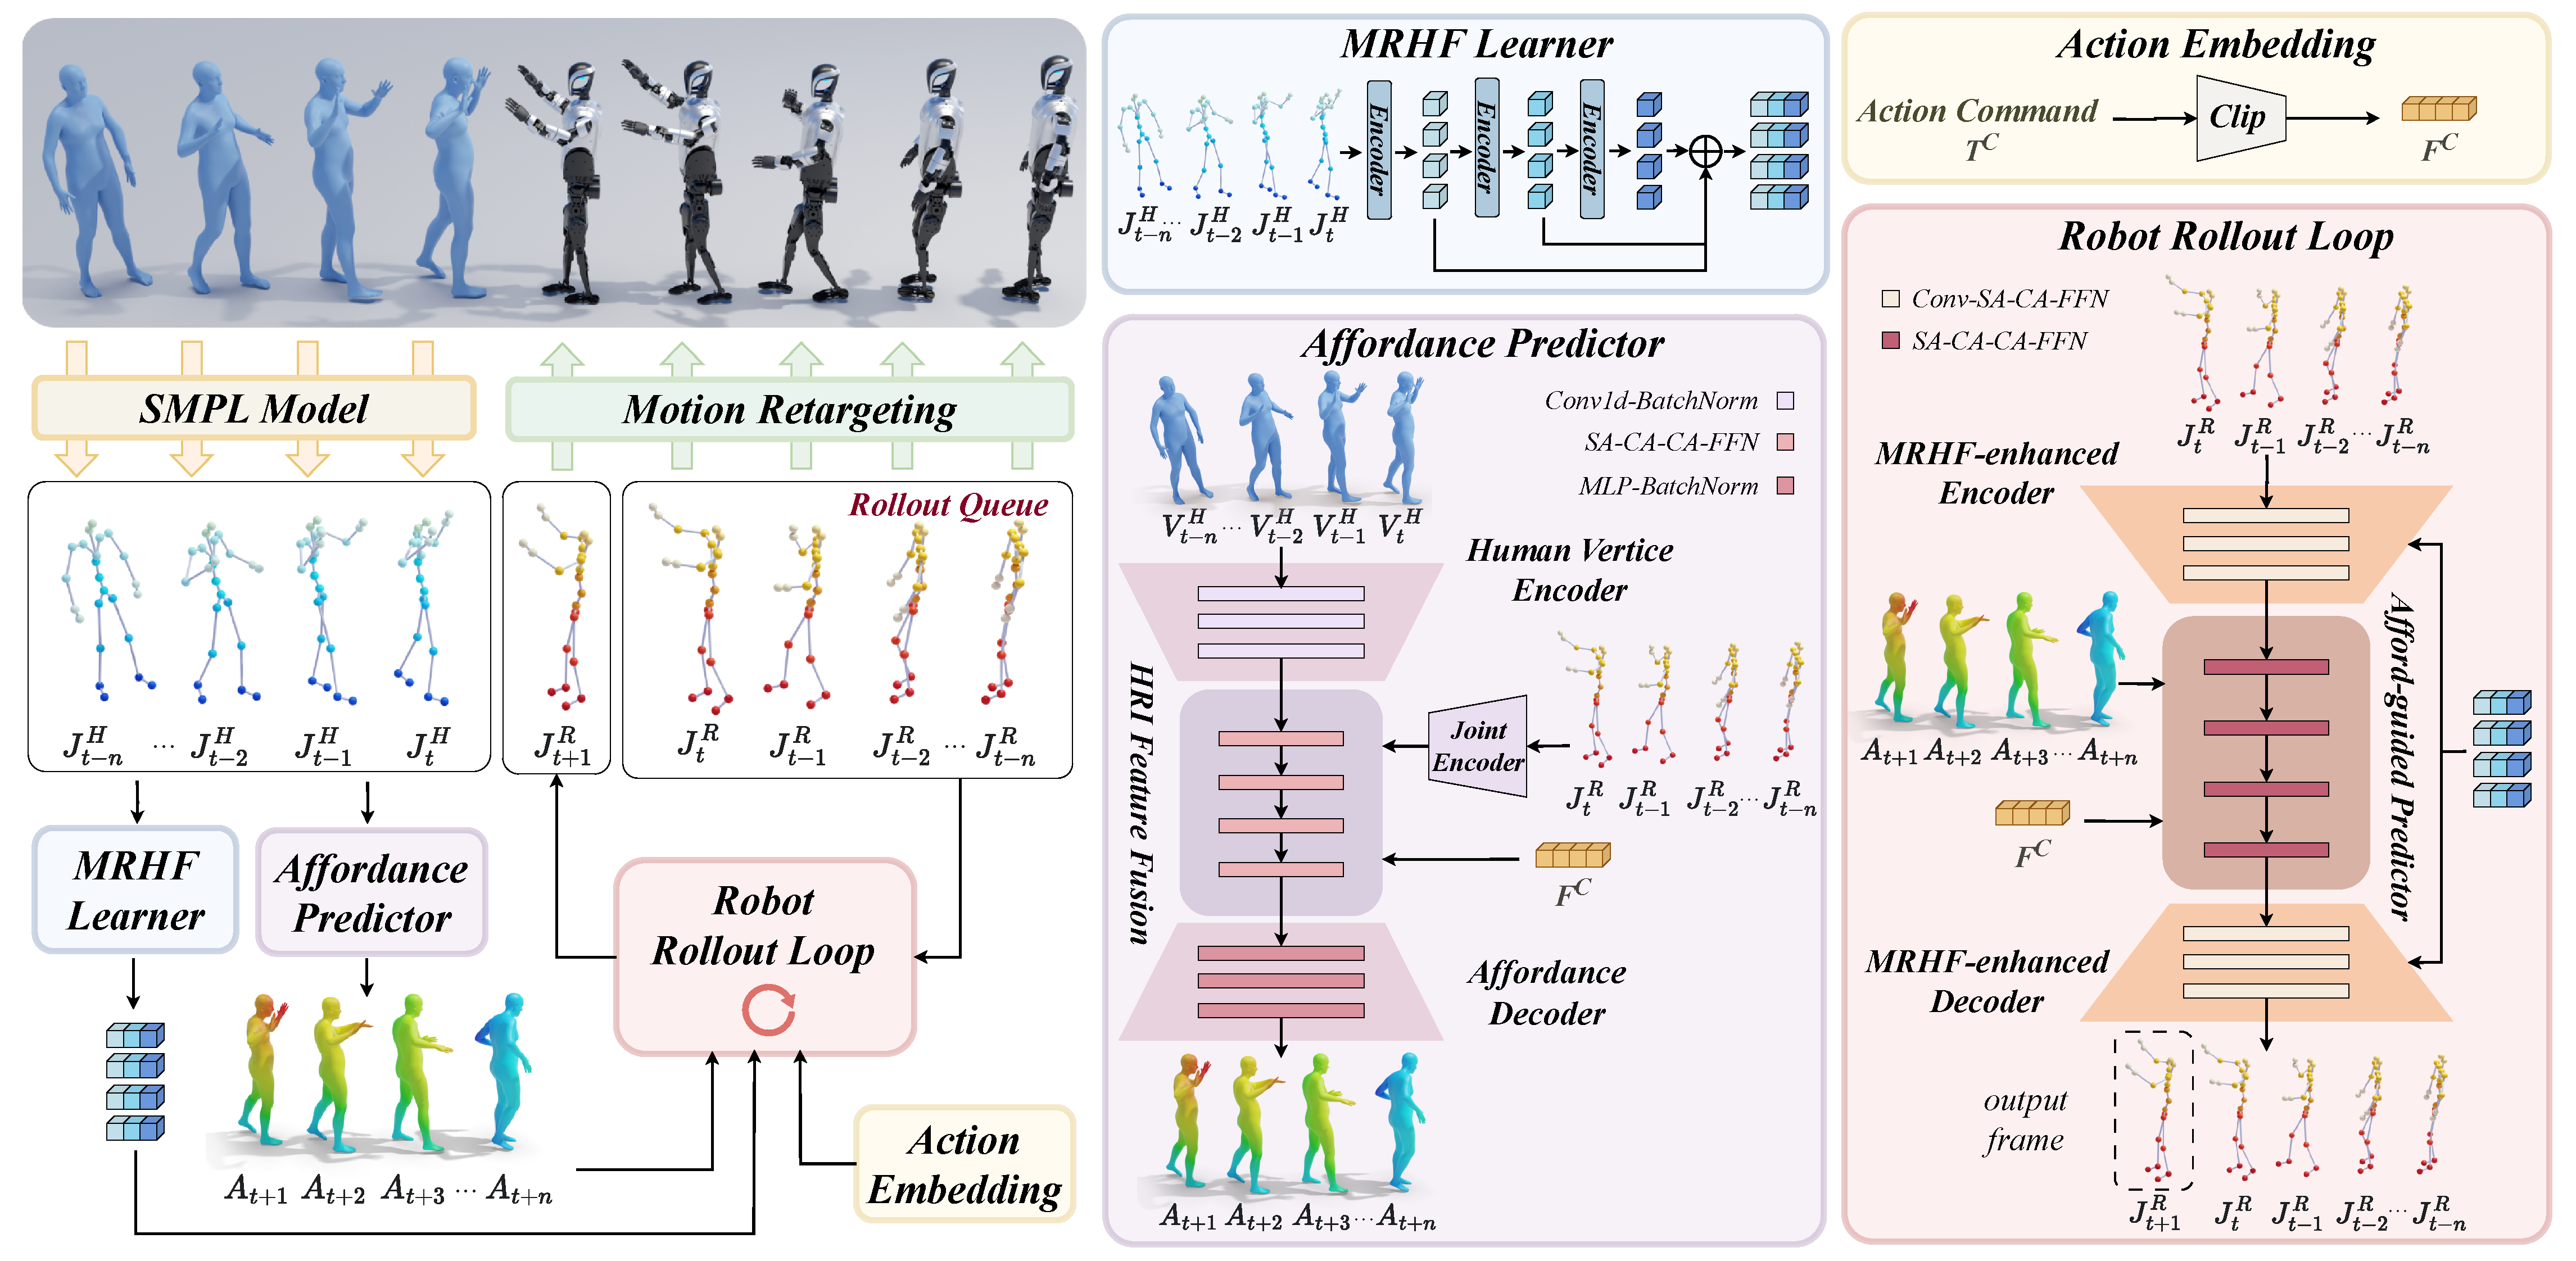
\includegraphics[width=1\linewidth]{images/intermodel-mainv5.pdf}
\vspace{-20pt}
\caption{Overall pipeline of our Robotic Interaction Model. The model ingests text action commands, historical robot joints, observed human joints and SMPL mesh vertices, and processes them through four tightly coupled modules. The Affordance Predictor explicitly estimates dense end-effector–vertex spatial fields to enable dexterous, socially-appropriate contact reasoning; the Multi-Resolution Human Feature (MRHF) Learner fuses hierarchical temporal cues to boost situational awareness; the Robot Rollout Loop leverages these affordance and human features to iteratively generate coherent, context-adaptive joint trajectories for real-time responsiveness; and finally, the Motion Retargeting module maps each predicted skeleton frame to robot-specific angle axis.}
\label{fig:interactiveModel}
\vspace{-10pt}
\end{figure*}